
\documentclass[11pt]{article}

\usepackage[margin=1in]{geometry}
\usepackage{amsmath, amssymb}
\usepackage{booktabs}
\usepackage{graphicx}
\usepackage{hyperref}
\usepackage{microtype}
\usepackage{enumitem}
\usepackage{amsthm}
\usepackage{tikz}
\usetikzlibrary{positioning,arrows.meta}

\newtheorem{proposition}{Proposition}


\title{Compression Efficiency and Structural Learning\\as a Computational Model of DLN Cognitive Stages}

\author{
Alia Wu\\
Risk Efficacy \& Redline Rising\\
\texttt{wut08@nyu.edu}\\
\href{https://orcid.org/0009-0005-4424-102X}{ORCID: 0009-0005-4424-102X}
}

\date{}

\begin{document}
\maketitle

\begin{abstract}
Extending the computational cognitive modeling tradition in which formal frameworks provide foundations for behavioral validation \cite{Marr1982,ACTR2004,KempTenenbaum2008}, we propose a computational instantiation of three cognitive stages from the Dot--Linear--Network (DLN) framework, grounded in a compression-efficiency thesis. DLN stages are characterized as graph-structured belief-dependency representations used to evaluate options: Dot as no persistent belief graph (reactive policies with negligible internal state), Linear as a null graph over option beliefs ($K$ independent option estimates with no information sharing), and Network as shared latent structure (a bipartite factor graph in which $F$ latent factors connect to $K$ options), augmented by a temporal exposure state and an explicit structural learning cycle (hypothesis $\rightarrow$ test $\rightarrow$ update/expand).

We formalize this cycle as navigation in a model space $\mathcal{M}$ whose
elements are candidate belief-dependency structures.  DLN stages are then
characterized by two formal objects: the belief-dependency graph $G$
(determining Level~1 inference cost) and a revision graph
$\mathcal{R}=(\mathcal{M},\mathcal{T})$ over $\mathcal{M}$ (determining Level~2
meta-cognitive capacity).  Linear cognition is a fixed point in $\mathcal{M}$
with $\mathcal{T}=\emptyset$; Network cognition revises by traversing edges of
$\mathcal{R}$, including a return transition that enables bounded recovery after
model failure.

In this mapping, Linear cognition learns and evaluates $K$ options independently ($O(K)$ cognitive cost), while Network cognition represents shared structure once ($O(F)$ cognitive cost for $F$ shared factors) and incorporates an explicit structural learning cycle: structural hypothesis $\rightarrow$ predictive test $\rightarrow$ update/expansion when the hypothesis fails.
We distinguish two compression targets: \emph{Option-factor structure} (shared structure in expected outcomes) and \emph{Stakes-factor structure} (shared structure in consequence-bearing exposures). Their intersection yields \emph{jointly efficient actions} that improve expected outcomes while simultaneously improving marginal stakes impact.
In a bandit-like simulation with factor-structured options and factor-structured stakes ($100$ seeds, $K\in\{20,50,100,200\}$, $F{=}5$, $T{=}80$), Network policies dominate Linear policies in cost-adjusted utility once the option set is sufficiently large (for example, at $K{=}200$ with stakes off, Network-Full achieves cost-adjusted utility $80.53$ vs.\ Linear $64.46$). We also derive an analytic crossover condition $K^* = F + c_{\mathrm{meta}}/c_{\mathrm{param}}$ that specifies when the fixed Level~2 overhead of revision is outweighed by Level~1 compression.
With stakes active, Linear policies incur large exposure penalties because they ignore covariance-induced cross-terms from cumulative exposure, while Network policies learn factor-level exposures and track cumulative exposure, maintaining positive utility (for example, at $K{=}200$ with stakes on, mean utility $66.78$ for Network vs.\ $-929.11$ for Linear).
These results evaluate internal consistency of a DLN-to-computation mapping under explicit assumptions; they do not validate a developmental theory in humans.
\end{abstract}











\section{Introduction}

Individuals can possess comparable amounts of domain knowledge yet differ sharply in \emph{how} that knowledge is organized and deployed. In practice, this manifests as differences in whether a person represents a situation as a set of disconnected facts, as a single privileged causal chain, or as an interacting system with feedback and cross-constraints. These differences matter for prediction, explanation, and decision support: two individuals can possess equivalent factual knowledge yet make systematically different choices because their internal representations differ in what they treat as shared, what they treat as independent, and how constraints propagate across elements. Making such structural differences explicit is relevant to human--AI interaction and cognitive modeling \cite{LakeEtAl2017}. In related traditions, this emphasis on feedback and cross-constraints is central to systems thinking \cite{Senge1990,Meadows2008}.

We propose the Dot--Linear--Network (DLN) framework, which treats such differences as differences in \emph{representational topology}: Dot as reactive processing without persistent belief structure, Linear as independent branch-by-branch estimation, and Network as shared latent structure with cross-branch information propagation. We employ graph-theoretic language: a cognitive state is represented as a graph $G=(V,E)$, where nodes are representational elements (concepts, features, action templates) and edges are statistical, causal, or constraint relations that allow information to propagate. Because ``topology'' can refer to multiple mathematical objects, we specify the relevant object precisely: our topological claims concern the agent's \emph{belief-dependency structure} used to evaluate options. In this framework, Dot corresponds to no persistent belief structure (reactive baselines), Linear corresponds to a null graph over $K$ option beliefs (independent option-by-option estimates with no edges), and Network corresponds to shared latent structure (options are d-connected through a smaller set of $F$ latent factors). Temporal coupling through cumulative exposure and a meta-level revision loop create feedback at the level of \emph{dynamics and learning}, even when the within-timestep belief graph is acyclic. This perspective complements existing work on knowledge graphs \cite{Hogan2021}, classic semantic-network and spreading-activation models \cite{CollinsLoftus1975,Anderson1983}, and cognitive architectures \cite{ACTR2004,Laird2012} by emphasizing that agents can differ not only in what they know, but in the qualitative dependency structure of what they know.

This paper focuses on a narrow computational thesis: \textbf{Network representations are structurally more efficient in stable environments because they represent shared components once rather than redundantly across each branch.} The central claim does not concern exploration-driven adaptation. Exploration strategies are well-studied in bandits and reinforcement learning \cite{Gershman2018,RussoBandits2018,SuttonBarto2018}; our focus is the representational \emph{reuse} mechanism that can render Network efficient even in stable environments. Robustness and adaptation can follow from the same mechanism, but the core test here is an efficiency scaling claim: do policies that represent shared structure once avoid $O(K)$ growth in representational and computational requirements as the number of options $K$ grows?

We decompose the thesis into two aligned compression targets. First, \emph{option-factor structure}: many options share components in their expected outcomes, so learning can be amortized across options if shared structure is represented (hierarchical shrinkage provides a classical example \cite{JamesStein1961,EfronMorris1977}). Second, \emph{stakes-factor structure}: the consequences of actions often share common drivers (exposure factors) in addition to idiosyncratic effects. When consequences are coupled through shared drivers, marginal impact depends on cumulative exposure, so a decision policy must represent cross-terms (covariances) rather than treating each action's stakes in isolation. The intersection of these structures makes \emph{jointly efficient actions} possible: a single action can be simultaneously beneficial for expected outcomes and beneficial for marginal stakes impact.

Mechanistically, we operationalize Network as a factorized model class coupled to an explicit structural learning cycle. The agent (i) begins with a compressed structural hypothesis, (ii) tests predictive adequacy against data, and (iii) expands or updates its hypothesis when it proves empirically inadequate. When the hypothesis is correct, the agent exploits compression and achieves $O(F)$-like scaling in the number of shared factors $F$; when the hypothesis fails, the agent pays additional cost to recover by expanding toward $O(K)$ state. This cycle constitutes the computational analogue of a structural prior $\rightarrow$ empirical test $\rightarrow$ revised prior mechanism.

\paragraph{Contributions.}
This paper contributes: (1) an explicit DLN-to-computation mapping centered on factorized compression rather than entropy-based exploration; (2) a stylized environment with option-factor structure, stakes-factor structure, and an explicit cross-term that makes cumulative exposure matter; (3) scaling results with paired-seed statistical summaries (bootstrap confidence intervals and paired effect sizes) identifying where compression helps and where it does not; and (4) an explicit assumption audit and reproducible code.

We emphasize scope: the simulation evaluates internal consistency of a proposed computational interpretation; it does not establish that human cognitive development follows DLN.


\section{DLN as a topological framework}

We model a cognitive state as a graph $G=(V,E)$ where nodes are representational elements (features, concepts, action templates) and edges are relations (associations, causal links, constraints). This section formalizes DLN stage distinctions as topological regimes.

\subsection{Topological regimes}

DLN is often summarized as Dot $\rightarrow$ Linear $\rightarrow$ Network, with increasingly connected representational graphs. Topology claims require specification of the object whose topology is being characterized. In this paper, the object is the agent's \emph{belief-dependency structure} used to evaluate options in a bandit-like setting (no explicit state transitions). The Linear stage thus corresponds to the simplest non-compressing representation: independent option-by-option estimation.

\paragraph{Dot stage (no persistent belief graph).}
Dot corresponds to policies with no persistent belief state for option evaluation. In our simulation, Dot selects uniformly at random and does not maintain outcome or exposure estimates.
Topologically, this corresponds to an empty (or ephemeral) belief graph: no stored nodes or edges allow information to propagate across options.

\paragraph{Linear stage (independent option beliefs; null belief graph).}
Linear corresponds to maintaining $K$ independent option beliefs (per-option means) with no edges between them.
Topologically, this is a null graph on $K$ belief nodes: no option shares an ancestor with any other option, so learning about option $i$ does not update beliefs about option $j$.
This captures the DLN property of branch-by-branch processing without reuse.

\paragraph{Network stage (shared latent structure; bipartite factor DAG).}
Network corresponds to representing options as arising from a smaller set of shared latent factors.
In our instantiation, the within-timestep belief graph is a bipartite directed acyclic graph (DAG): $F$ latent factor nodes connect to $K$ option nodes.
Options that share a factor share an ancestor and are therefore d-connected through the factor; evidence from one option updates the factor belief, which updates predicted values for all factor-mates.
This shared-parent structure is the graph-theoretic source of integration in our implementation: shared structure represented once and reused across many options.

\paragraph{Where cycles enter: dynamics and meta-learning.}
Although the factor belief graph is a DAG, Network-stage cognition in DLN is also associated with feedback and revisitation.
In this paper, those notions correspond to (i) a closed-loop dependency in the \emph{system dynamics} when stakes are active (actions update exposure $E_t$, and $E_t$ feeds back into the marginal penalty term used to evaluate future actions), and (ii) a \emph{process-level} structural learning cycle (hypothesis $\rightarrow$ test $\rightarrow$ update/expand) that revises which belief graph is being used.

Section~\ref{sec:model_space} formalizes this distinction by defining a model
space $\mathcal{M}$ whose elements are candidate belief structures and a
revision graph $\mathcal{R}$ whose edges are transitions between them; the cycle
that defines Network cognition is a structural feature of $\mathcal{R}$, not of
any individual belief graph $G\in\mathcal{M}$.

This distinction is necessary to avoid conflating graph structure with inference complexity: the present claim is not that cyclic belief graphs enable cheaper inference than trees. Rather, investing in shared latent structure can reduce the number of distinct quantities that must be learned from $K$ to $F$ when the structure hypothesis is correct.

\subsection{Cost-scaling interpretation}

The computational claim tested here is a scaling distinction:
\begin{itemize}[leftmargin=*]
\item \textbf{Dot:} no accumulation of learning across encounters (reactive; baseline).
\item \textbf{Linear:} independent estimation per option, yielding complexity that scales with the number of options $K$.
\item \textbf{Network:} factorized representation that learns a smaller number of shared factors $F$ and propagates factor updates to many options, yielding complexity that scales primarily with $F$ rather than $K$.
\end{itemize}


\paragraph{Formal complexity statement.}
Let Linear maintain per-option sufficient statistics $(\widehat{\mu}_i,n_i)$ for $i\in\{1,\dots,K\}$.
Then its representational state requires
\[
M_{\mathrm{Lin}}(K)=\Theta(K).
\]
In our implementation, Linear also scores all options each step, yielding per-decision computation
$G_{\mathrm{Lin}}(K)=\Theta(K)$.
Let Network maintain per-factor statistics $(\widehat{m}_f,\widehat{b}_f,n_f)$ for $f\in\{1,\dots,F\}$ plus the exposure state $E_t$, and use a bounded within-factor local search of size $L$ (treated as a constant).
Then
\[
M_{\mathrm{Net}}(F)=\Theta(F)+\Theta(1),\qquad
G_{\mathrm{Net}}(F)=\Theta(F+L)=\Theta(F)\ \text{for fixed }L.
\]
When the factor hypothesis fails and the model expands to a tabular representation, Network reverts to $\Theta(K)$ state and computation.
Thus the compression thesis predicts an advantage only when $F\ll K$ \emph{and} the factor hypothesis remains empirically adequate; when $K=F$ (no shared components), the advantage should vanish, constituting a falsification criterion for the compression thesis.

\begin{proposition}[Cost separation and recovery bound]\label{prop:crossover}
Let an agent face a $K$-option decision environment with $F$-factor structure
($F \leq K$).  Let $c_{\mathrm{param}}$ be the per-element parameter learning
cost and $c_{\mathrm{meta}}$ be the Level~2 model-revision overhead (navigation
of the revision graph $\mathcal{R}$, Section~\ref{sec:model_space}).  Then:

\begin{enumerate}[label=(\roman*)]
\item \textbf{Crossover.}
For $K < K^* = F + c_{\mathrm{meta}}/c_{\mathrm{param}}$, Linear achieves lower
total cognitive cost than Network (Network cannot do better than operating in a
correct compressed model and still paying its Level~2 overhead).
For $K > K^*$, Network under a correct factor hypothesis achieves lower total
cost by replacing $O(K)$ per-episode parameter maintenance with $O(F)$, up to the
fixed overhead $c_{\mathrm{meta}}$.

\item \textbf{Catastrophic failure under cross-terms.}
When the environment contains stakes-factor structure with covariance coupling,
Linear's utility degrades without bound in cumulative exposure $E_t$ because it
cannot represent the marginal penalty term $2E_t b_i$.  Network's utility
remains bounded because it tracks $E_t$ and computes marginal impact.

\item \textbf{Recovery bound.}
When the factor hypothesis is incorrect and the agent expands to
$G_{\mathrm{tab}}$, an agent whose revision graph $\mathcal{R}$ includes a
return transition $(G_{\mathrm{tab}}, G_F) \in \mathcal{T}$ recovers $O(F)$ cost
scaling within $n_{\mathrm{contract}} + w + n_{\mathrm{converge}}$ steps after
factor structure becomes present, where $n_{\mathrm{converge}}$ is the number of
observations required for within-factor variance to fall below the contraction
threshold.  An agent without a return transition (expand-only Network or Linear)
remains at $O(K)$ cost indefinitely.
\end{enumerate}

Parts (i) and (ii) are tested by the existing simulation results.
Part (iii) is tested by the contraction ablation
(Section~\ref{sec:contraction}).
\end{proposition}

\paragraph{Proof sketch for (i).}
In the absence of structural sharing, Linear must maintain $K$ parameters, so
its per-episode cost is proportional to $c_{\mathrm{param}}K$.  A Network agent
that is operating in a correct compressed model maintains only $F$ parameters,
but still pays a fixed Level~2 overhead $c_{\mathrm{meta}}$ for monitoring and
revision.  Comparing $c_{\mathrm{param}}K$ against $c_{\mathrm{param}}F +
c_{\mathrm{meta}}$ yields the crossover condition $K^* = F +
c_{\mathrm{meta}}/c_{\mathrm{param}}$.

\paragraph{Proof sketch for (ii).}
Under stakes, the true marginal impact of choosing option $i$ contains a
cross-term proportional to $2E_t b_i$, where $E_t$ is cumulative exposure.  A
Linear agent that treats options independently can include a per-option penalty
(e.g., $\lambda b_i^2$) but cannot represent the coupling to $E_t$, so it cannot
stabilize exposure as $|E_t|$ grows.  A Network agent that tracks $E_t$ and
computes marginal impact can keep exposure bounded, preventing unbounded penalty
growth.

\paragraph{Proof sketch for (iii).}
After expanding to $G_{\mathrm{tab}}$, an agent with a return transition can
periodically test whether a compressed factor model predicts well again (for
example via a length-$w$ evaluation window after a holdout period
$n_{\mathrm{contract}}$).  Once factor structure is present and sufficient data
are accumulated ($n_{\mathrm{converge}}$ observations), the agent contracts back
to $G_F$ and returns to $O(F)$ scaling.  Without a return transition, the agent
remains in the expanded model and continues to incur $O(K)$ cost.


This relates to classical results on shrinkage and hierarchical estimation: when structure exists, sharing statistical strength across related items improves efficiency \cite{JamesStein1961,EfronMorris1977}. In our mapping, Network operationalizes this by tracking factor-level beliefs and using them to score options, while retaining the capacity to expand to option-specific state when structure is violated.

\subsection{Factor structure as a computational analogue of network integration}

The computational instantiation used here is intentionally simple: Network is represented as a shared factor space. This is not meant to claim that human cognition is a literal factor model, but it renders the topology-to-computation mapping concrete. If we represent each option $i$ as connected to a factor node $c_i$, then the representational graph becomes a bipartite structure in which many options share the same factor node. Updating the factor belief propagates immediately to all connected options. This is precisely the ``represent shared components once'' property that DLN attributes to integrated (network-stage) organization.

Stakes-factor structure adds an additional coupling: the current exposure state $E_t$ links sequential decisions, and the marginal stakes impact contains a cross-term $2E_tb_i$. This introduces a feedback-like dependency across time: the consequences of an action depend on what has been selected before. A Linear representation that evaluates stakes per option without tracking $E_t$ treats this dependency as if it were absent; a Network representation explicitly represents the coupling and therefore computes marginal impact. In this minimal setting, the coupling induces closed-loop decision dynamics: the state induced by prior actions feeds back into the evaluation of future actions.

This mapping implies a design requirement: to test DLN Network as integrated structure, the environment must contain shared components and cross-constraints that make reuse and coupling beneficial. If structure is absent or if $K=F$ (no shared components), the representation should not help. Those boundary tests are part of the falsifiable surface of the thesis.




\subsection{Model space and revision graph}\label{sec:model_space}

The preceding sections characterize DLN stages by the within-episode
belief-dependency graph $G$ that an agent uses to represent outcomes, exposures,
and option relations.  Our Network instantiation also implements an explicit
structural learning cycle that can \emph{revise which belief graph is active}
when a structural hypothesis fails.  To formalize this two-level distinction, we
separate (i) inference and learning \emph{within} a belief graph (Level~1) from
(ii) monitoring and revising the belief graph itself (Level~2).

\paragraph{Model space.}
Let $\mathcal{M}$ be a set of candidate belief-dependency structures.  In the
present instantiation, the core model space contains two elements:
a compressed factor graph $G_F$ (shared latent factors connecting options) and
an expanded tabular graph $G_{\mathrm{tab}}$ (independent option beliefs).
Formally, $\mathcal{M}=\{G_F,\,G_{\mathrm{tab}}\}$.

\paragraph{Revision graph.}
Define the \emph{revision graph} as a directed graph over model space,
$\mathcal{R}=(\mathcal{M},\mathcal{T})$, where $\mathcal{T}\subseteq
\mathcal{M}\times\mathcal{M}$ is the set of revision transitions available to an
agent.  In our simulation, the key transitions are:
(i)~\emph{expansion} (switching from $G_F$ to $G_{\mathrm{tab}}$ when the factor
hypothesis fails) and (ii)~\emph{contraction} (switching from $G_{\mathrm{tab}}$
back to $G_F$ when predictive evidence supports compression again).

\paragraph{Completing the cycle: contraction.}
Expansion alone yields an irreversible path $G_F \rightarrow
G_{\mathrm{tab}}$.  Adding a contraction transition
$(G_{\mathrm{tab}},G_F)\in\mathcal{T}$ completes a revision cycle.  This return
transition matters even when $|\mathcal{M}|=2$: it is the mechanism that
enables an agent to recover compressed $O(F)$ operation after a period of
operating in an expanded $O(K)$ representation.

\paragraph{Revision capacity by DLN stage.}
The revision graph characterizes each stage's meta-cognitive capacity in
graph-combinatorial terms:
%
\begin{itemize}[leftmargin=*]
\item \textbf{Dot.}  No model space ($|\mathcal{M}|=0$); $\mathcal{R}$
  is empty.  No revision capacity.
\item \textbf{Linear.}  $\mathcal{M} = \{G_{\mathrm{tab}}\}$; a single
  vertex with no edges.  The agent occupies a fixed point in model space.
\item \textbf{Network (expand-only).}  $\mathcal{M} =
  \{G_F, G_{\mathrm{tab}}\}$; one directed edge
  $G_F \to G_{\mathrm{tab}}$.  The agent can detect model failure and
  expand, but cannot return to a compressed representation.
\item \textbf{Network (full cycle).}  Two directed edges (expand and
  contract).  $\mathcal{R}$ contains a cycle: the agent can depart from a
  model, operate under an alternative, and return.  This is the
  graph-theoretic signature of full revision capacity.
\end{itemize}
%
The functional consequence of the return transition is stated in
Proposition~\ref{prop:crossover}(iii): an agent that can return to
$G_F$ recovers $O(F)$ cost scaling in bounded time; an agent that
cannot is permanently locked at $O(K)$.

\paragraph{Two levels of computation.}
Level~1 computation concerns inference and parameter learning within a chosen
belief graph $G\in\mathcal{M}$ (e.g., updating factor means or option means).
Level~2 computation concerns monitoring model adequacy and executing transitions
in $\mathcal{R}$.  Proposition~\ref{prop:crossover}(iii) establishes that an
agent whose revision graph includes a return transition recovers $\Theta(F)$
scaling in bounded time once factor structure is present, while an agent without
a return transition remains at $\Theta(K)$ permanently.

\paragraph{Relationship to the tractable-cognition literature.}
Work on probabilistic graphical models and treewidth analyzes the complexity of
inference \emph{within a fixed model structure} \cite{Pearl1988,vanRooij2008,Kwisthout2010}.
Our claims are different in kind: we focus on when representing shared
structure reduces the number of distinct quantities an agent must learn from $K$
to $F$, and on what revision transitions are required to recover that advantage
after model failure.


\begin{figure}[t]
  \centering
  \begin{minipage}[t]{0.56\linewidth}
    \centering
    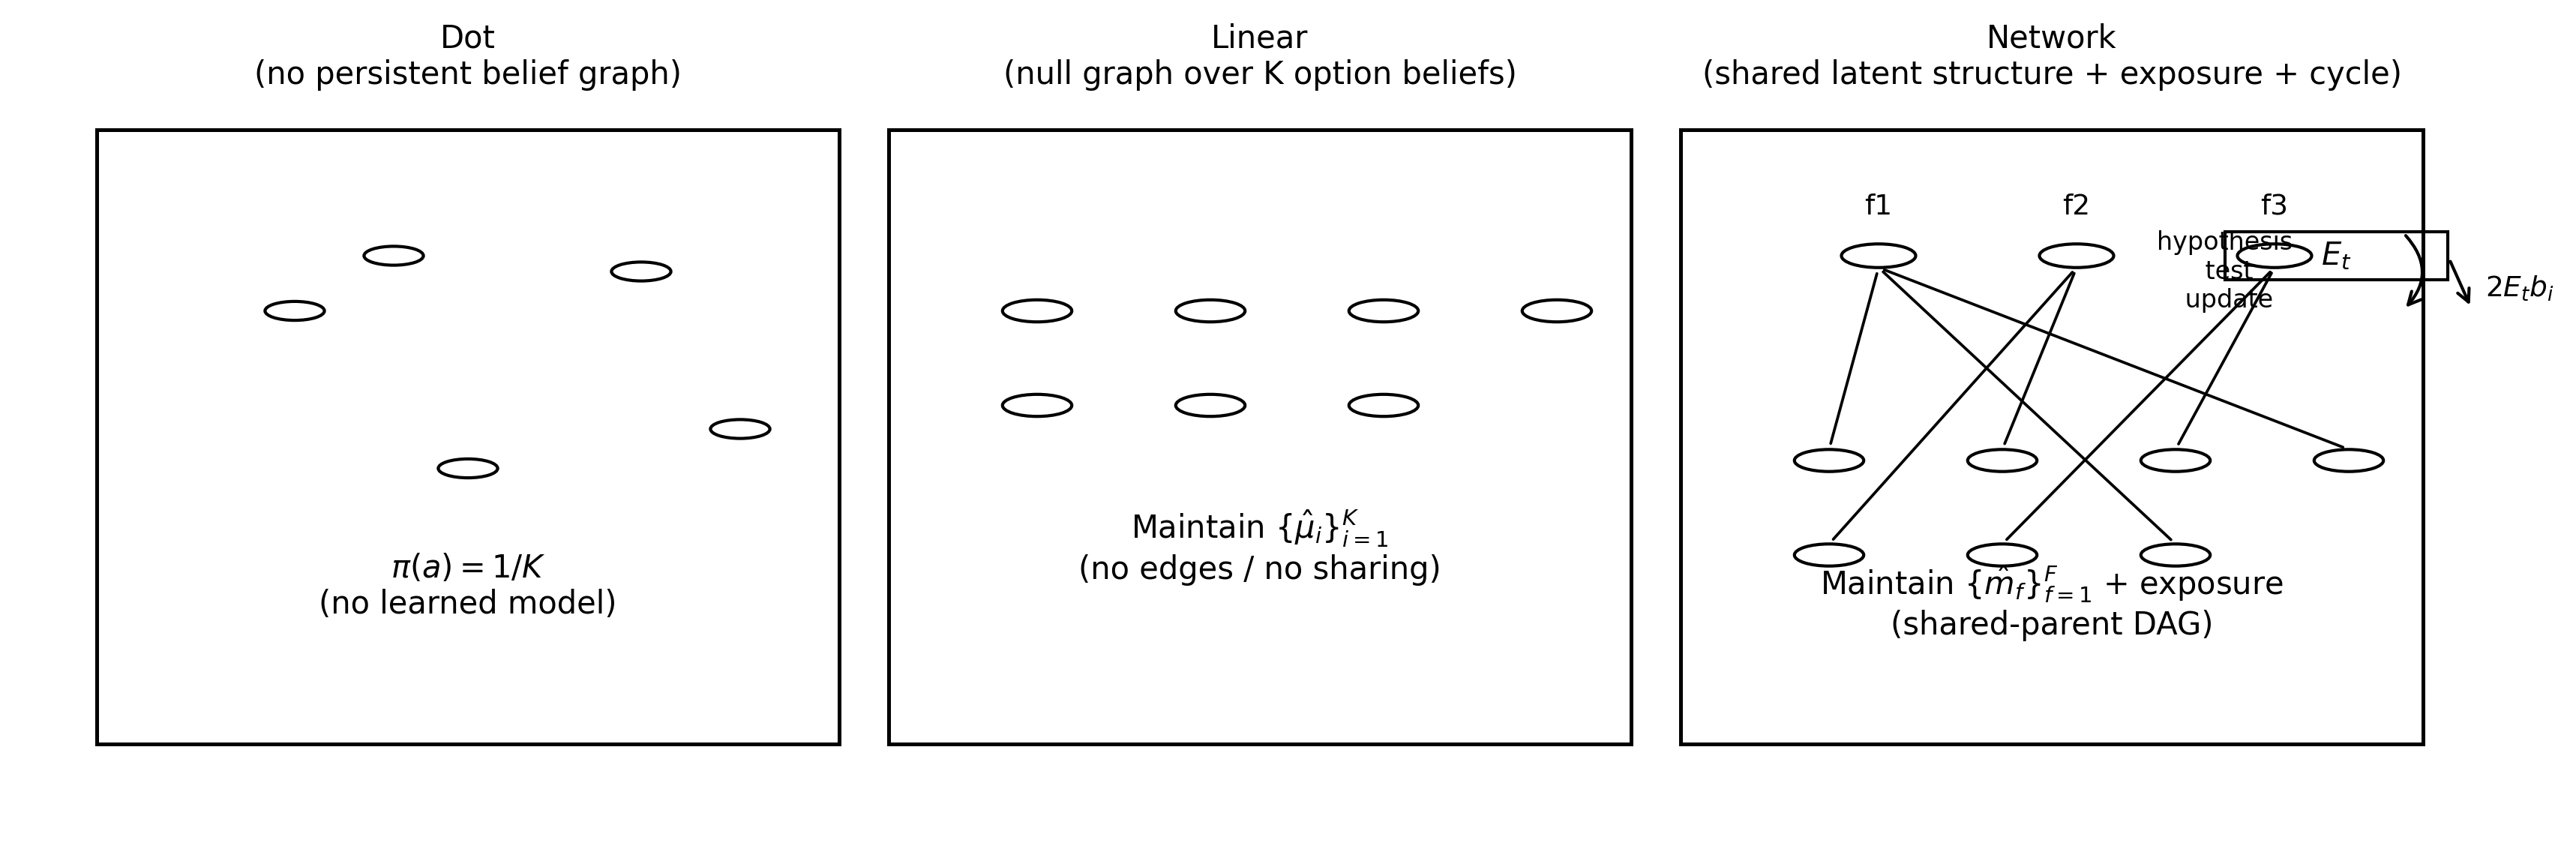
\includegraphics[width=\linewidth]{figures/fig_dln_topology.png}
    \vspace{0.5ex}

    {\small\textbf{(a)} Belief-dependency structures (Level~1).}
  \end{minipage}\hfill
  \begin{minipage}[t]{0.41\linewidth}
    \centering
    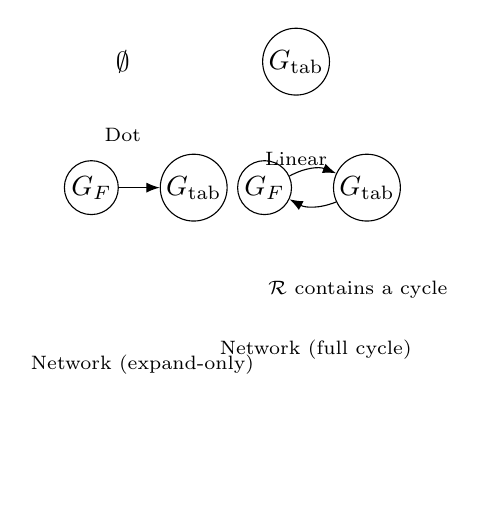
\begin{tikzpicture}[
        >=Latex,
        every node/.style={circle,draw,inner sep=1pt,minimum size=0.55cm},
      ]
      % Dot
      \node[draw=none] (dot) at (0,0) {$\emptyset$};
      \node[draw=none, below=0.35cm of dot] {\scriptsize Dot};

      % Linear
      \node (lin) at (2.2,0) {$G_{\mathrm{tab}}$};
      \node[draw=none, below=0.35cm of lin] {\scriptsize Linear};

      % Network (expand-only)
      \node (gF1) at (-0.4,-1.6) {$G_F$};
      \node (gT1) at (0.9,-1.6) {$G_{\mathrm{tab}}$};
      \draw[->] (gF1) -- (gT1);
      \node[draw=none, below=0.35cm of gT1, xshift=-0.65cm] {\scriptsize Network (expand-only)};

      % Network (full cycle)
      \node (gF2) at (1.8,-1.6) {$G_F$};
      \node (gT2) at (3.1,-1.6) {$G_{\mathrm{tab}}$};
      \draw[->] (gF2) to[bend left=25] (gT2);
      \draw[->] (gT2) to[bend left=25] (gF2);
      \node[draw=none, below=0.35cm of gT2, xshift=-0.65cm] {\scriptsize Network (full cycle)};

      \node[draw=none, below=0.95cm of gF2, anchor=west] {\scriptsize $\mathcal{R}$ contains a cycle};
    \end{tikzpicture}
    \vspace{0.5ex}

    {\small\textbf{(b)} Revision graphs over model space (Level~2).}
  \end{minipage}

  \caption{
(a) Belief-dependency structures (Level~1). Dot: no persistent graph.
Linear: null graph on $K$ option nodes. Network: bipartite factor DAG with $F$
factor nodes connected to $K$ options.
(b) Revision graphs over model space (Level~2). Dot: empty model space.
Linear: fixed point in model space (no revision edges).
Network (expand-only): directed path $G_F \rightarrow G_{\mathrm{tab}}$.
Network (full cycle): two directed transitions (expand and contract) forming a
cycle in $\mathcal{R}$, enabling bounded recovery
(Proposition~\ref{prop:crossover}(iii)).
}
  \label{fig:dln_topology}
\end{figure}



\section{Claims and predictions}

\subsection{Problem framing}

We separate three claims.

\paragraph{(C1) Option-factor structure compression.}
Options share components. A Network-stage policy learns shared structure once and reuses it across many options (effective cost scaling with $F$), while a Linear-stage policy learns each option independently (effective cost scaling with $K$).

\paragraph{(C2) Stakes-factor structure compression.}
Consequence-bearing exposures share components. A Network-stage policy learns common exposure structure and tracks cumulative exposure so that a single hedge can reduce a shared driver once, rather than repeatedly per option. A Linear-stage policy treats exposures as independent and therefore misses covariance-driven marginal effects.

\paragraph{(C3) Intersection: jointly efficient actions.}
Actions can be simultaneously beneficial on expected outcomes (Option-factor structure) and beneficial on marginal exposure impact (Stakes-factor structure). A Network-stage policy can identify these overlaps because both decompositions are represented in a shared factor space.


\subsection{Diagnostic signatures}

The computational mapping yields diagnostic signatures that are testable in simulations (as demonstrated here) and, in principle, in behavioral experiments:

\begin{itemize}[leftmargin=*]
\item \textbf{Scaling signature (reuse vs.\ redundancy).} In tasks with option-factor structure, regret or cost-adjusted utility should scale primarily with the number of factors $F$ under Network representations but with the number of options $K$ under Linear representations.
\item \textbf{Marginal-stakes signature.} When consequences depend on cumulative exposure (covariance cross-terms), Network policies should behave as if evaluating \emph{marginal} impact given current exposure state, while Linear policies behave as if evaluating each option's consequences independently.
\item \textbf{Intersection signature (jointly efficient actions).} When option-factor and stakes-factor structure overlap, Network policies should identify actions that serve both objectives simultaneously more reliably than Linear policies, especially when the overlap is sparse.
\item \textbf{Prior failure signature (recovery vs.\ silent degradation).} Under prior-wrong conditions, Network policies should exhibit measurable model updates (switches/expansions) and improved fit relative to no-test or no-update ablations, at the cost of increased cognitive cost.
\end{itemize}

These signatures separate the compression thesis from generic claims of adaptation or exploration. In particular, the scaling signature should obtain in stable environments without distribution shift.
Each signature yields quantitative predictions testable in human behavioral experiments: option-set size manipulations can identify the crossover point, process-tracing methods can distinguish marginal-stakes evaluation from independent evaluation, and response-time scaling can dissociate factor-level from option-level processing.


\subsection{Explicit assumptions}

We state assumptions explicitly, as they determine the scope of claims the simulation can support.

\begin{itemize}[leftmargin=*]
  \item \textbf{A1 (observed option-factor labels).} Each option $i$ has an observed option-factor label $c_i\in\{0,\dots,F-1\}$. This stands in for a shared-component representation. (Linear agents choose to ignore it.)
  \item \textbf{A2 (observed stakes loading).} Each option exposes an observed stakes loading $b_i\in\mathbb{R}$.
  \item \textbf{A3 (structured outcomes; prior correct).} In the structured condition, mean outcomes follow a factor model: $\mu_i = m_{c_i} + \epsilon_i$.
  \item \textbf{A4 (unstructured outcomes; prior wrong).} In the unstructured condition, $\mu_i$ are independent and the label $c_i$ is irrelevant for predicting outcome.
  \item \textbf{A5 (stakes objective and covariance cross-term).} Stakes are represented as a quadratic exposure objective in a 1D exposure state $E_t$. Selecting option $i$ updates exposure $E_{t+1}=E_t+b_i$ and incurs incremental penalty
  \[
  \Delta P_t = \lambda\left((E_t+b_i)^2 - E_t^2\right)=\lambda(2E_tb_i+b_i^2).
  \]
  The cross-term $2E_tb_i$ is the minimal mechanism by which cumulative exposure creates marginal effects that cannot be captured by option-by-option penalty terms alone.
  \item \textbf{A6 (cognitive cost proxy).} We use an algorithmic proxy cost consisting of memory units and compute units with weights (reported in the run manifest). This is a complexity surrogate, not a claim about biological energy.
\end{itemize}


\begin{table}[t]
\caption{Assumption audit: what is built in, and relaxation paths.}
\label{tab:assumption_audit}
\centering
\begin{tabular}{p{0.08\linewidth} p{0.55\linewidth} p{0.12\linewidth} p{0.18\linewidth}}
\toprule
ID & Assumption (informal) & Built-in? & Relaxation path \\
\midrule
A1 & Factor label $c_i$ is observed (shared-component index). & Yes & Learn $c_i$ / latent factors via clustering or representation learning. \\
A2 & Stakes loading $b_i$ is observed. & Yes & Learn $b_i$ (or exposures) from observed consequences. \\
A3 & Structured outcomes follow $\mu_i=m_{c_i}+\epsilon_i$. & Swept & Sweep structure strength (within-factor variance). \\
A4 & Unstructured outcomes violate the factor prior (prior wrong). & Swept & Add partial structure and drifting structure regimes. \\
A5 & Stakes penalty contains cross-term via exposure state $E_t$. & Yes & Move to multi-dimensional $E_t$ and general quadratic forms. \\
A6 & Cognitive cost is a proxy based on memory/compute scaling. & Yes & Sensitivity analysis; report Pareto frontiers instead of a single $\alpha$. \\
\bottomrule
\end{tabular}
\end{table}

\begin{table}[t]
\caption{Claim-to-test matrix: what each experiment condition identifies.}
\label{tab:claim_matrix}
\centering
\begin{tabular}{p{0.16\linewidth} p{0.26\linewidth} p{0.52\linewidth}}
\toprule
Claim & Condition & Observable signature \\
\midrule
C1 (Option-factor compression) & Structured, stakes$=0$, sweep $K$ & Network surpasses Linear at large $K$ in cost-adjusted utility; Linear cost grows with $K$ while Network cost is $\approx O(F)$. \\
C2 (Stakes-factor compression) & Structured, stakes$>0$, sweep $K$ & Linear utility degrades substantially due to unmodeled exposure cross-terms; Network remains stable by tracking cumulative exposure and using marginal impact. \\
C3 (Intersection) & Structured, stakes$>0$ & Network selects jointly efficient actions (high outcome, favorable marginal stakes) at a higher rate than Linear, especially when overlap is sparse. \\
Recovery (prior wrong) & Unstructured, stakes$=0$ (and $>0$) & Network-Full shows switch/expansion events and outperforms NoTest/NoUpdate ablations, paying increased cognitive cost. \\
Boundary (no compression) & $K=F$ & Network advantage disappears (falsifier for compression thesis). \\
\bottomrule
\end{tabular}
\end{table}


\section{Relationship to existing work}

\subsection{Cognitive architectures and bounded rationality}

DLN is not intended to replace established cognitive theories or architectures, but to provide a structural lens that can complement them. Many cognitive architectures specify symbolic or production-system mechanisms \cite{ACTR2004,Laird2012}, and many modern AI systems operationalize relational knowledge as graphs \cite{Hogan2021}. The present contribution emphasizes that belief-dependency structure imposes computational constraints. When option beliefs are independent, evidence updates a single option; when options share latent structure, evidence propagates through shared parents, allowing one observation to update many options. This constitutes a representational and statistical-generalization claim rather than a claim about the computational cost of cyclic belief graphs.

DLN also connects to bounded rationality traditions in which limited computational resources necessitate simplified representations \cite{Simon1955,TverskyKahneman1974,GigerenzerGoldstein1996}. In this paper, the resource constraint is made explicit as a cognitive cost proxy and a scaling claim: Linear representations are expensive because they duplicate estimation across options, while Network representations can amortize learning across options when shared structure exists.

From a developmental perspective, stage theories often describe qualitative shifts in what operations become possible \cite{Piaget1952,Kegan1994}. The distinctive DLN claim is not about specific content operations, but about a shift in representational topology that makes certain computations cheaper (reuse) and makes others less likely (redundant branch-by-branch processing). Dynamic-systems accounts emphasize that qualitative shifts can emerge from continuous changes in coupling strength and feedback \cite{ThelenSmith1994}; the structural learning cycle instantiated here is compatible with that view because it creates a mechanism by which representational coupling is strengthened when it explains data and relaxed when it fails.


\subsection{Computational neuroscience: structure learning as a distinct operation}

Computational neuroscience and cognitive science have repeatedly distinguished between (i) \emph{structure learning} (selecting, constructing, or revising a latent representation such as latent causes, task sets, or structural forms) and (ii) \emph{parameter learning} (updating values within a chosen representation).
Gershman and Niv \cite{GershmanNiv2010} review how inferring latent structure can support rapid generalization beyond what tabular reinforcement learning can provide, and Collins and Frank \cite{CollinsFrank2013} model when learners create and reuse task-set structure rather than only fitting parameters within a fixed task representation.
From a broader cognitive-science perspective, Kemp and Tenenbaum \cite{KempTenenbaum2008} demonstrate that humans can infer different \emph{structural forms} from data, and hierarchical Bayesian accounts formalize when abstraction accelerates learning by sharing statistical strength across related instances \cite{Gershman2017}.
Work on cognitive control and arbitration similarly emphasizes cost--benefit tradeoffs in deploying more computationally demanding strategies, including when model-based control becomes worthwhile \cite{Kool2016}.

Neural evidence is consistent with this two-level distinction.
Causal and structure learning signals have been reported in frontoparietal networks that are at least partially dissociable from striatal value-learning signals \cite{Tomov2018}.
Related work suggests that frontopolar and rostrolateral prefrontal cortex can compute reliability over alternative strategies or learning systems \cite{Lee2014} and can support reasoning over counterfactual strategies not currently deployed \cite{Koechlin2014}.
We do not claim a neural implementation in this paper; we cite these results only to motivate treating structure learning as a distinct computational operation rather than folding it into parameter learning.

Building on this foundation, our contribution is more circumscribed: we instantiate DLN stage differences as differences in \emph{belief-dependency structure} and derive a concrete efficiency prediction for a particular representational family.
First, we make the scaling implication of shared latent structure explicit as an $O(F)$ versus $O(K)$ crossover (Section~2.2), where $F$ is the number of shared factors and $K$ is the number of options.
Second, we extend the same compression logic to \emph{stakes-factor structure} by introducing an exposure objective with an explicit covariance cross-term, so that the marginal consequence of an action depends on cumulative exposure state.
Third, we connect these representational regimes to a three-stage DLN mapping (Dot/Linear/Network) and test falsifiers and ablations (e.g., $K{=}F$ and prior-wrong conditions) that isolate when the structural learning cycle matters.

This positioning also clarifies how our claims relate to graph-theoretic complexity results.
Classical work on probabilistic graphical models \cite{Pearl1988} and the treewidth / tractable-cognition literature \cite{vanRooij2008,Kwisthout2010} analyze the complexity of inference \emph{within a fixed model structure} and establish that low-treewidth graphs enable efficient inference.
The within-timestep belief graph for the Network agent is itself a low-treewidth bipartite DAG; we do not claim that cycles in belief graphs make inference cheaper than trees.
Instead, we focus on a representation-construction question: when the world admits shared structure with $F\ll K$ and the factor hypothesis is empirically adequate, representing shared structure reduces the number of distinct quantities that must be learned from $K$ to $F$; when structure is absent or incorrect, expansion toward a tabular representation removes the advantage.

\paragraph{Formalizing the gap.}
The structure-learning literature distinguishes learning \emph{within} a chosen
representation from learning \emph{which} representation to use (or when to
switch) \cite{KempTenenbaum2008,CollinsFrank2013}.  Section~\ref{sec:model_space}
makes this distinction explicit in our DLN instantiation: Level~1 computation
occurs within a belief-dependency graph $G\in\mathcal{M}$, while Level~2
computation is navigation in the revision graph $\mathcal{R}$ over model space.
The crossover $K^* = F + c_{\mathrm{meta}}/c_{\mathrm{param}}$
(Proposition~\ref{prop:crossover}(i)) makes precise when paying a fixed Level~2
overhead is cost-effective relative to the $O(F)$ savings from representing
shared structure.




\section{Simulation design}

\subsection{Structural learning cycle}

The Network stage is not defined merely by the presence or absence of structure. It is defined as an explicit revision cycle over a small model space (Section~\ref{sec:model_space}):
\begin{enumerate}[leftmargin=*]
  \item \textbf{Structural hypothesis (compressed prior).} Start with a compressed factor hypothesis for outcome prediction in $G_F$.
  \item \textbf{Predictive test.} Maintain a rolling window of factor prediction errors (mean squared error over the last $W$ steps). If the rolling error exceeds an expansion threshold $\tau_{\mathrm{expand}}$, treat this as evidence that the factor hypothesis is inadequate.
  \item \textbf{Expansion on mismatch.} On mismatch, expand to a tabular representation $G_{\mathrm{tab}}$ (allocate per-option outcome estimates). This removes compression but restores predictive adequacy when the factor hypothesis is wrong.
  \item \textbf{Contraction (return transition).} While operating in the expanded model, periodically test whether a compressed factor model can again predict well. After a holdout period $n_{\mathrm{contract}}$, open an evaluation window of length $w$ in which the agent runs a \emph{shadow} factor model, initialized from current tabular estimates (group means over options that share a factor). If the shadow factor model satisfies
  $\mathrm{MSE}_{\mathrm{shadow}} < (1-\theta_{\mathrm{contract}})\mathrm{MSE}_{\mathrm{tab}}$,
  the agent contracts back to $G_F$ and (optionally) frees tabular state, returning memory scaling to $O(F)$.
\end{enumerate}

This constitutes a concrete implementation of a structural prior $\rightarrow$ test $\rightarrow$ revised prior mechanism: the hypothesis is the factor predictor, the test is a rolling-window predictive check, and the revised hypothesis is represented by transitions in the revision graph (expansion $G_F\!\rightarrow\!G_{\mathrm{tab}}$ and contraction $G_{\mathrm{tab}}\!\rightarrow\!G_F$).

We report three Network ablations that isolate components of this Level~2 cycle: Network-NoTest disables the predictive check; Network-NoUpdate runs the check but disallows transitions; Network-NoContract allows expansion but disables the return transition, making revision irreversible once the model expands.


\subsection{Environment}

We use a bandit-like environment with $K$ options and $F$ factors. Each option $i$ carries a factor label $c_i$. Outcomes are Gaussian:
\[
r_t \sim \mathcal{N}(\mu_{a_t}, \sigma_r^2).
\]
In the structured (prior-correct) condition, $\mu_i=m_{c_i}+\epsilon_i$ with small idiosyncratic noise; in the unstructured (prior-wrong) condition, the $\mu_i$ are independent. Stakes loadings are factor-structured:
\[
b_i = g_{c_i} + \delta_i,
\]
with small idiosyncratic noise. Utility is the sum of outcomes minus incremental stakes penalties.

\subsection{Agents}

\textbf{Dot.} The Dot agent selects uniformly at random and performs no learning.

\textbf{Linear.} The Linear agent maintains tabular frequentist mean estimates per option; action selection scores each option using a local stakes heuristic that ignores the cross-term $2E_tb_i$:
\[
\text{score}(i) = \widehat{\mu}_i - \lambda b_i^2.
\]
This scoring function treats hedging as separable across options and does not track cumulative exposure.\footnote{A hybrid ``Linear+$E_t$'' agent could track cumulative exposure while maintaining independent option beliefs. We exclude this design because tracking $E_t$ requires representing how past choices affect future evaluations---a cross-option temporal dependency inconsistent with the branch-by-branch independence that characterizes Linear-stage cognition. Isolating the factor-compression and exposure-tracking contributions via such an ablation is a direction for future work.}

\textbf{Network-Full.} The Network-Full agent maintains factor-level outcome estimates $\widehat{m}_f$ and factor-level exposure estimates $\widehat{b}_f$, tracks $E_t$, and uses the true marginal penalty form. Within a chosen factor, Network searches over at most $L{=}5$ options to avoid hiding $O(K)$ scans in factor selection. It also runs the predictive check, can expand to tabular outcome estimates when the factor hypothesis fails, and can contract back to the factor model when predictive evidence supports compression again (completing a return transition in the revision graph).

\textbf{Ablations.} Network-NoTest disables the predictive check; Network-NoUpdate runs the check but disallows model-class transitions; Network-NoContract allows expansion but disables the return transition to the compressed model.

\subsection{Metrics and statistics}

Per episode we report:
(i) total outcome, (ii) total stakes penalty, (iii) utility $U=\sum_t (r_t-\Delta P_t)$,
(iv) cognitive cost proxy $C$, (v) cost-adjusted utility $U-\alpha C$,
(vi) jointly efficient action pick count, (vii) number of expansion transitions $G_F\rightarrow G_{\mathrm{tab}}$,
(viii) number of contraction (return) transitions $G_{\mathrm{tab}}\rightarrow G_F$, and
(ix) time spent in each model class (steps in $G_F$ vs.\ $G_{\mathrm{tab}}$).

Results are averaged over $100$ random seeds with paired comparisons across seeds (same environment seed per agent). For key paired differences we report bootstrap $95\%$ confidence intervals (percentile bootstrap over seeds) and paired Cohen's $d$ on the seed-wise difference.

\section{Results}

\subsection{Option-factor structure compression (Claim C1)}

Table~\ref{tab:cau_struct0} reports cost-adjusted utility in the stable structured environment (stakes off). As $K$ grows, Linear cognitive cost scales with $K$, while Network cost is approximately constant in $F$ (Table~\ref{tab:cog_scaling}). Network overtakes Linear for larger option sets: at $K=200$, Network-Full achieves cost-adjusted utility $80.53$ vs.\ Linear $64.46$ (paired difference mean $+16.08$).

\subsection{Stakes-factor structure compression (Claim C2)}

With stakes active, Linear agents incur large penalties because they do not represent the cross-term $2E_tb_i$ and cannot hedge cumulative exposure. Network agents track $E_t$ and learn factor-level exposure structure, enabling hedging and keeping penalty bounded. At $K=200$ in the structured setting, Network-Full maintains positive mean utility ($66.78$) while Linear incurs substantial negative utility ($-929.11$). The paired utility difference is $+995.89$.


\subsection{Dot baseline}

Dot serves as the null-graph baseline: it does not accumulate value estimates, does not represent option-factor or stakes-factor structure, and does not track cumulative exposure $E_t$. As a result, Dot does not benefit from increasing $K$ even when option-factor structure is present. In the stable structured setting with stakes off (Table~\ref{tab:cau_struct0}), Dot's cost-adjusted utility remains near zero across $K$ (means between $-0.51$ and $0.88$), reflecting near-chance outcomes combined with near-zero cognitive cost.

With stakes active (Table~\ref{tab:util_struct1}), Dot incurs negative utility (roughly $-57$ to $-109$) because cumulative exposure follows an uncontrolled random walk. Dot avoids Linear's extreme degradation only because it also avoids systematic exploitation; this reflects robustness through non-commitment rather than compression. Network differs by maintaining positive utility while simultaneously optimizing outcomes and controlling marginal exposure impact.


\subsection{Jointly efficient actions (Claim C3)}

In the structured stakes condition, the environment contains a sparse set of actions that are \emph{jointly efficient} by construction: they are high on expected outcome \emph{and} reduce marginal exposure impact under the stakes objective.
Formally, the true incremental penalty for selecting option $i$ at exposure state $E_t$ is
\[
\Delta P_t(i)=\lambda\left((E_t+b_i)^2-E_t^2\right)=\lambda(2E_tb_i+b_i^2),
\]
so the \emph{marginal} stakes contribution depends on the sign interaction between the cumulative exposure $E_t$ and the option's loading $b_i$.
A jointly efficient action is one that simultaneously has high $\mu_i$ and (when $E_t$ is positive) has $b_i<0$ so that the cross-term $2E_tb_i$ is negative.

\paragraph{Evaluation definition.}
At environment initialization we flag a small subset of options as jointly efficient (the \texttt{dual\_mask}): options in the top reward quantile that also have negative exposure loading.
This flag is computed from the environment's ground-truth $(\mu_i,b_i)$ and is fixed \emph{before} any agent acts.
We report the pick rate as the fraction of timesteps in which the chosen action lies in this flagged set (Figure~\ref{fig:joint}).

\paragraph{Why intersection requires representing both decompositions.}
To identify a jointly efficient action, a policy must (i) know which actions are promising on expected outcomes (Option-factor structure) and (ii) evaluate \emph{marginal} stakes impact given current exposure $E_t$ (Stakes-factor structure).
Network-Full represents both: it learns factor-level outcome estimates, learns factor-level exposure estimates, tracks $E_t$, and scores factors/actions using the true marginal form.
Linear fails on (ii): it uses a local stakes heuristic $\widehat{\mu}_i-\lambda b_i^2$ that ignores the cross-term and the sign interaction with $E_t$, so it systematically undervalues actions that are beneficial precisely because their exposure loading offsets existing exposure.
Dot fails on both (i) and (ii) because it is non-learning and exposure-agnostic.

\subsection{Prior-wrong condition: the learning cycle expands the model}

In the unstructured condition, the factor hypothesis for outcome prediction is incorrect. Network-Full allocates tabular state (expansion) and improves raw utility relative to NoTest/NoUpdate ablations, while paying an explicit cognitive cost for doing so. For example at $K=200$ (unstructured, stakes off), Network-Full exceeds Network-NoTest by $+7.31$ utility (bootstrap $95\%$ CI $[2.23,12.66]$) and exceeds Network-NoUpdate by $+8.50$ (bootstrap $95\%$ CI $[3.65,13.54]$), while exhibiting more hypothesis expansions (Figure~\ref{fig:switches}).

\paragraph{Interpreting the ablations.}
Network-NoTest corresponds to compression without validation: it trusts the factor hypothesis unconditionally and therefore continues pooling across irrelevant labels when the prior is incorrect, accumulating systematic bias.
Network-NoUpdate corresponds to validation without adaptation: it allocates computation (and may even allocate tabular state for comparison) to detect mismatch, but is not permitted to switch its action model, so it pays overhead without recovering performance.
Network-Full requires both the predictive test and the update/expansion branch to recover under prior failure; the performance gaps in the unstructured condition demonstrate that the \emph{learning cycle} (not just factorization) is performing work.


\begin{figure}[t]
  \centering
  
\includegraphics[width=0.95\linewidth]{figures/fig_cau_vs_K_structured_stakes0.0.png}
  \caption{Stable structured environment (stakes=0): cost-adjusted utility vs.\ number of options $K$ for Dot, Linear, and Network-Full.}
  \label{fig:core}
\end{figure}

\begin{figure}[t]
  \centering
  
\includegraphics[width=0.95\linewidth]{figures/fig_cau_vs_K_structured_stakes1.0.png}
  \caption{Structured environment with stakes (stakes=1): cost-adjusted utility vs.\ $K$. Linear incurs substantial negative utility due to unmodeled cumulative exposure; Network maintains utility by tracking $E_t$ and using marginal impact.}
  \label{fig:stakes}
\end{figure}

\begin{figure}[t]
  \centering
  
\includegraphics[width=0.95\linewidth]{figures/fig_dual_purpose_rate.png}
  \caption{Jointly efficient action pick rate (structured, stakes=1).}
  \label{fig:joint}
\end{figure}

\begin{figure}[t]
  \centering
  
\includegraphics[width=0.75\linewidth]{figures/fig_switches.png}
  \caption{Prior-wrong condition (unstructured, stakes=0): mean number of hypothesis expansions (switches) for Network variants.}
  \label{fig:switches}
\end{figure}


\begin{table}[t]
\caption{Cost-adjusted utility (mean $\pm$ sd) in the stable structured environment (stakes=0).}
\label{tab:cau_struct0}
\centering
\begin{tabular}{rlll}
\toprule
$K$ & Dot & Linear & Network-Full \\
\midrule
20 & 0.88 $\pm$ 9.99 & 86.31 $\pm$ 34.59 & 83.21 $\pm$ 35.27 \\
50 & $-$1.25 $\pm$ 8.64 & 83.03 $\pm$ 34.07 & 86.25 $\pm$ 33.41 \\
100 & $-$0.46 $\pm$ 9.03 & 81.76 $\pm$ 35.60 & 82.67 $\pm$ 37.32 \\
200 & $-$0.22 $\pm$ 8.69 & 64.46 $\pm$ 31.73 & 80.53 $\pm$ 33.90 \\
\bottomrule
\end{tabular}
\end{table}

\begin{table}[t]
\caption{Cognitive cost proxy (mean $\pm$ sd) showing $O(K)$ scaling for Linear and $O(F)$ scaling for Network.}
\label{tab:cog_scaling}
\centering
\begin{tabular}{rll}
\toprule
$K$ & Linear & Network-Full \\
\midrule
20 & 2.27 $\pm$ 0.04 & 1.68 $\pm$ 0.07 \\
50 & 5.07 $\pm$ 0.13 & 1.75 $\pm$ 0.02 \\
100 & 9.73 $\pm$ 0.25 & 1.75 $\pm$ 0.02 \\
200 & 19.05 $\pm$ 0.50 & 1.75 $\pm$ 0.02 \\
\bottomrule
\end{tabular}
\end{table}

\begin{table}[t]
\caption{Utility (mean $\pm$ sd) in the structured environment with stakes (stakes=1).}
\label{tab:util_struct1}
\centering
\begin{tabular}{rlll}
\toprule
$K$ & Dot & Linear & Network-Full \\
\midrule
20 & $-$108.65 $\pm$ 145.49 & $-$1132.80 $\pm$ 1616.31 & 72.28 $\pm$ 35.44 \\
50 & $-$107.71 $\pm$ 138.95 & $-$919.45 $\pm$ 1462.16 & 64.65 $\pm$ 34.10 \\
100 & $-$68.02 $\pm$ 83.13 & $-$1006.74 $\pm$ 1412.20 & 69.18 $\pm$ 33.07 \\
200 & $-$74.77 $\pm$ 101.39 & $-$929.11 $\pm$ 1537.36 & 66.78 $\pm$ 29.62 \\
\bottomrule
\end{tabular}
\end{table}


\subsection{Contraction and bounded recovery (return transition)}\label{sec:contraction}

The prior-wrong condition above isolates why the Network stage must include
\emph{expansion}: when the factor hypothesis fails, an agent that remains in
$G_F$ is locked into a mis-specified compressed representation.  Completing the
revision cycle requires an additional capability: once compression becomes
appropriate again, the agent must be able to return to $G_F$.

To isolate this return transition, we include Network-NoContract, which is
identical to Network-Full except that it disables contraction
($G_{\mathrm{tab}}\rightarrow G_F$).  We evaluate Network-Full and
Network-NoContract in a recovery setting that forces initial expansion and then
makes compression appropriate again.  The key measurements are
(i)~the number of contraction (return) events,
(ii)~the number of contraction evaluation windows opened, and
(iii)~the fraction of steps spent in $G_F$ versus $G_{\mathrm{tab}}$.
These measurements directly test Proposition~\ref{prop:crossover}(iii): an agent
whose revision graph includes a return transition should recover $\Theta(F)$
scaling in bounded time after factor structure becomes present, whereas an
agent without a return transition remains at $\Theta(K)$ cost scaling.


\section{Discussion}

\subsection{Interpretation}

Under Assumptions A1--A6, the simulation isolates the efficiency consequences of representing shared structure. Dot is included as the null-graph baseline (no accumulation, no compression) to anchor the three-stage ordering; it is expected to ignore both structure and stakes. The simulation does \emph{not} establish whether humans actually represent options and exposures in this way. Developmental interpretations are also potentially culturally contingent; see WEIRD-sampling cautions \cite{Henrich2010}. The revision graph $\mathcal{R}$ introduced in Section~\ref{sec:model_space} provides a formal model of this deployment layer: the structural learning cycle implements Level~2 computation (navigation of $\mathcal{R}$), and the crossover condition $K^* = F + c_{\mathrm{meta}}/c_{\mathrm{param}}$ determines when investing in Level~2 is cost-effective.  This connects to metacognitive monitoring \cite{Flavell1979,Bandura1997} by formalizing what is monitored (model adequacy, via predictive tests) and what actions are available in response (transitions in $\mathcal{R}$).

\paragraph{Meta-cognition as a property of model space.}
DLN stages differ not only in the structure of the belief graph $G$ (Level~1) but
in whether the agent can navigate a non-trivial model space (Level~2).  Linear
cognition is a fixed point in $\mathcal{M}$.  Network cognition traverses
$\mathcal{M}$ via revision transitions, including a return transition whose
functional consequence is bounded cost recovery after model failure
(Proposition~\ref{prop:crossover}(iii)).  This provides a foundation for
instantiating DLN in other domains: any system where an observer, agent, or
learner can be characterized by (i)~a current representational structure and
(ii)~a set of available transitions between structures can be classified by
the structure of its revision graph.


The compression-efficiency thesis tested here is distinct from exploration-driven adaptation; the Network advantage obtains in stable environments without requiring distribution shift or novelty-seeking (Section~1). Exploration mechanisms are well-studied elsewhere \cite{Gershman2018,RussoBandits2018}; our focus is the representational reuse that makes compression beneficial even when the environment is stationary.

\subsection{Boundary conditions}

The results depend on explicit structural gaps between $K$ and $F$ and on the presence of cross-terms in the stakes objective.

\paragraph{When $K=F$ (no compression available).}
If every option is its own factor, then there is no shared component to compress. In that case, a Network factor representation should offer no advantage over Linear, and may perform worse due to representational overhead. This constitutes a key falsifier for the compression thesis.

\paragraph{Partial structure.}
If option-factor structure is weak (large within-factor deviations), the benefit of shrinkage and factor scoring should degrade smoothly. Likewise for stakes-factor structure: if exposures are not aligned with factors, the hedging benefit should degrade. A structure-strength sweep makes these boundary conditions visible.

\paragraph{Stakes scaling versus stakes structure.}
This paper models stakes through \emph{structured exposures} with a covariance-inducing cross-term. Scaling stakes magnitude alone is a different question; both can be studied, but they test different mechanisms.

\subsection{Limitations and future work}

\paragraph{Observed factor labels (A1).}
We assume the Network agent has access to a shared-component representation $c_i$. This provides a representational advantage rather than requiring the agent to learn it.
\emph{Future direction:} replace $c_i$ with learned clustering or learned latent factors (Bayesian nonparametrics or representation learning) and report the additional sample and cognitive costs required to learn the representation.

\paragraph{1D exposure state (A5).}
We use a single exposure dimension to make the cross-term explicit and interpretable.
\emph{Future direction:} extend to $d$-dimensional exposures with $E_t\in\mathbb{R}^d$ and penalty $\|E_t\|^2$ (or a quadratic form $E_t^\top \Sigma E_t$). Measure how Network cost scales with the number of exposure factors rather than with the number of options.

\paragraph{Cognitive cost proxy (A6).}
We use an algorithmic proxy (memory and compute scaling).
\emph{Future direction:} perform sensitivity analysis over cost weights and $\alpha$, and report Pareto frontiers over (utility, cost) rather than a single calibrated point estimate.

\paragraph{Local search within factor.}
Network uses a bounded local search of size $L$ within a chosen factor to avoid hiding $O(K)$ scans.
\emph{Future direction:} vary $L$ (ablation) to quantify the tradeoff between factor-level compression and within-factor deviation exploitation.

\paragraph{Decomposing compression and exposure tracking.}
The present design confounds two mechanisms: factor-level compression (representing shared structure once) and cumulative exposure tracking (using $E_t$ to compute marginal impact). A Linear agent augmented with $E_t$-tracking but no factor structure would isolate these contributions.
\emph{Future direction:} implement a ``Linear+$E_t$'' baseline and measure how much of the stakes-condition advantage (Claim C2) arises from compression versus exposure tracking.


\section{Reproducibility}\label{sec:repro}

All tables in this paper are derived from \texttt{outputs/paper/results/episode\_metrics.csv}. The default run that reproduces the CSV and baseline figures is:

\begin{verbatim}
python src/dln_core_variable_cycle.py --preset paper --out outputs/paper
\end{verbatim}

The run writes \texttt{outputs/paper/results/manifest.json} containing hyperparameters, seeds, and file hashes. Baseline figures are written under \texttt{outputs/paper/artifacts/figures/}. To regenerate figures with different styling, use the CSV as the single source of truth and rebuild plots externally.

\paragraph{Code availability.}
The complete source code, simulation framework, and reproducibility scripts are available at:
\url{https://github.com/aliawu08/dln-compression-model}


\section{Conclusion}

Two formal objects carry the DLN distinction: the belief-dependency graph $G$,
whose structure determines Level~1 inference cost, and the revision graph
$\mathcal{R}$ over model space, whose structure determines Level~2 meta-cognitive
capacity.  Linear cognition is a fixed point in model space; Network cognition
navigates $\mathcal{R}$ via hypothesis, test, and revision transitions.
Proposition~\ref{prop:crossover} derives the crossover
$K^* = F + c_{\mathrm{meta}}/c_{\mathrm{param}}$ from the interaction between
Level~1 compression and Level~2 overhead, and shows that including a return
transition in $\mathcal{R}$ provides bounded recovery after model failure.
This two-object characterization provides a foundation for instantiating DLN in
domains beyond decision-making, including settings where representational
constraints determine what information an agent can extract from its
environment.

\begin{thebibliography}{99}

\bibitem{Anderson1983}
J.~R. Anderson.
\newblock \emph{The Architecture of Cognition}.
\newblock Harvard University Press, 1983.

\bibitem{ACTR2004}
J.~R. Anderson, D.~Bothell, M.~D. Byrne, S.~Douglass, C.~Lebiere, and Y.~Qin.
\newblock An integrated theory of the mind.
\newblock \emph{Psychological Review}, 111(4):1036--1060, 2004.

\bibitem{Bandura1997}
A.~Bandura.
\newblock \emph{Self-Efficacy: The Exercise of Control}.
\newblock W.\,H. Freeman, 1997.

\bibitem{CollinsLoftus1975}
A.~M. Collins and E.~F. Loftus.
\newblock A spreading-activation theory of semantic processing.
\newblock \emph{Psychological Review}, 82(6):407--428, 1975.

\bibitem{CollinsFrank2013}
A.~G.~E. Collins and M.~J. Frank.
\newblock Cognitive control over learning: creating, clustering, and generalizing task-set structure.
\newblock \emph{Psychological Review}, 120(1):190--229, 2013.

\bibitem{EfronMorris1977}
B.~Efron and C.~Morris.
\newblock Stein's paradox in statistics.
\newblock \emph{Scientific American}, 236(5):119--127, 1977.

\bibitem{Flavell1979}
J.~H. Flavell.
\newblock Metacognition and cognitive monitoring: a new area of cognitive-developmental inquiry.
\newblock \emph{American Psychologist}, 34(10):906--911, 1979.

\bibitem{Gershman2017}
S.~J. Gershman.
\newblock On the blessing of abstraction.
\newblock \emph{The Quarterly Journal of Experimental Psychology}, 70(3):361--365, 2017.

\bibitem{Gershman2018}
S.~J. Gershman.
\newblock Deconstructing the human algorithms for exploration.
\newblock \emph{Cognition}, 173:34--42, 2018.

\bibitem{GershmanNiv2010}
S.~J. Gershman and Y.~Niv.
\newblock Learning latent structure: carving nature at its joints.
\newblock \emph{Current Opinion in Neurobiology}, 20(2):251--256, 2010.

\bibitem{GigerenzerGoldstein1996}
G.~Gigerenzer and D.~G. Goldstein.
\newblock Reasoning the fast and frugal way: models of bounded rationality.
\newblock \emph{Psychological Review}, 103(4):650--669, 1996.

\bibitem{Henrich2010}
J.~Henrich, S.~J. Heine, and A.~Norenzayan.
\newblock The weirdest people in the world?
\newblock \emph{Behavioral and Brain Sciences}, 33(2--3):61--83, 2010.

\bibitem{Hogan2021}
A.~Hogan, E.~Blomqvist, M.~Cochez, C.~d'Amato, G.~de~Melo, C.~Gutierrez, \emph{et~al.}
\newblock Knowledge graphs.
\newblock \emph{ACM Computing Surveys}, 54(4):1--37, 2021.

\bibitem{JamesStein1961}
W.~James and C.~Stein.
\newblock Estimation with quadratic loss.
\newblock In \emph{Proceedings of the Fourth Berkeley Symposium on Mathematical Statistics and Probability}, pages 361--379. University of California Press, 1961.

\bibitem{Kegan1994}
R.~Kegan.
\newblock \emph{In Over Our Heads: The Mental Demands of Modern Life}.
\newblock Harvard University Press, 1994.

\bibitem{KempTenenbaum2008}
C.~Kemp and J.~B. Tenenbaum.
\newblock The discovery of structural form.
\newblock \emph{Proceedings of the National Academy of Sciences}, 105(31):10687--10692, 2008.

\bibitem{Koechlin2014}
E.~Koechlin.
\newblock An evolutionary computational theory of prefrontal executive function in decision-making.
\newblock \emph{Philosophical Transactions of the Royal Society B}, 369(1655):20130474, 2014.

\bibitem{Kool2016}
W.~Kool, F.~A. Cushman, and S.~J. Gershman.
\newblock When does model-based control pay off?
\newblock \emph{PLoS Computational Biology}, 12(8):e1005090, 2016.

\bibitem{Kwisthout2010}
J.~Kwisthout, T.~Wareham, and I.~van Rooij.
\newblock The necessity of bounded treewidth for efficient inference in {B}ayesian networks.
\newblock In \emph{Proceedings of the 19th European Conference on Artificial Intelligence (ECAI)}, pages 237--242, 2010.

\bibitem{Laird2012}
J.~E. Laird.
\newblock \emph{The Soar Cognitive Architecture}.
\newblock MIT Press, 2012.

\bibitem{Marr1982}
D.~Marr.
\newblock \emph{Vision: A Computational Investigation into the Human Representation and Processing of Visual Information}.
\newblock W.\,H. Freeman, 1982.

\bibitem{LakeEtAl2017}
B.~M. Lake, T.~D. Ullman, J.~B. Tenenbaum, and S.~J. Gershman.
\newblock Building machines that learn and think like people.
\newblock \emph{Behavioral and Brain Sciences}, 40:e253, 2017.

\bibitem{Lee2014}
S.~W. Lee, S.~Shimojo, and J.~P. O'Doherty.
\newblock Neural computations underlying arbitration between model-based and model-free learning.
\newblock \emph{Neuron}, 81(3):687--699, 2014.

\bibitem{Meadows2008}
D.~H. Meadows.
\newblock \emph{Thinking in Systems: A Primer}.
\newblock Chelsea Green Publishing, 2008.

\bibitem{Pearl1988}
J.~Pearl.
\newblock \emph{Probabilistic Reasoning in Intelligent Systems: Networks of Plausible Inference}.
\newblock Morgan Kaufmann, 1988.

\bibitem{Piaget1952}
J.~Piaget.
\newblock \emph{The Origins of Intelligence in Children}.
\newblock International Universities Press, 1952.

\bibitem{RussoBandits2018}
D.~Russo, B.~Van~Roy, A.~Kazerouni, I.~Osband, and Z.~Wen.
\newblock A tutorial on {T}hompson sampling.
\newblock \emph{Foundations and Trends in Machine Learning}, 11(1):1--96, 2018.

\bibitem{Senge1990}
P.~M. Senge.
\newblock \emph{The Fifth Discipline: The Art and Practice of the Learning Organization}.
\newblock Doubleday, 1990.

\bibitem{Simon1955}
H.~A. Simon.
\newblock A behavioral model of rational choice.
\newblock \emph{The Quarterly Journal of Economics}, 69(1):99--118, 1955.

\bibitem{SuttonBarto2018}
R.~S. Sutton and A.~G. Barto.
\newblock \emph{Reinforcement Learning: An Introduction}.
\newblock MIT Press, 2nd edition, 2018.

\bibitem{ThelenSmith1994}
E.~Thelen and L.~B. Smith.
\newblock \emph{A Dynamic Systems Approach to the Development of Cognition and Action}.
\newblock MIT Press, 1994.

\bibitem{Tomov2018}
M.~S. Tomov, H.~M. Dorfman, and S.~J. Gershman.
\newblock Neural computations underlying causal structure learning.
\newblock \emph{Journal of Neuroscience}, 38(32):7143--7157, 2018.

\bibitem{TverskyKahneman1974}
A.~Tversky and D.~Kahneman.
\newblock Judgment under uncertainty: heuristics and biases.
\newblock \emph{Science}, 185(4157):1124--1131, 1974.

\bibitem{vanRooij2008}
I.~van Rooij.
\newblock The tractable cognition thesis.
\newblock \emph{Cognitive Science}, 32(6):939--984, 2008.

\end{thebibliography}

\end{document}
